%%%%%%%%%%%%%%%%%%%%%%%%%%%%%%%%%%%%%%%%%
% Thin Sectioned Essay
% LaTeX Template
% Version 1.0 (3/8/13)
%
% This template has been downloaded from:
% http://www.LaTeXTemplates.com
%
% Original Author:
% Nicolas Diaz (nsdiaz@uc.cl) with extensive modifications by:
% Vel (vel@latextemplates.com)
%
% License:
% CC BY-NC-SA 3.0 (http://creativecommons.org/licenses/by-nc-sa/3.0/)
%
%%%%%%%%%%%%%%%%%%%%%%%%%%%%%%%%%%%%%%%%%

%----------------------------------------------------------------------------------------
%	PACKAGES AND OTHER DOCUMENT CONFIGURATIONS
%----------------------------------------------------------------------------------------

\documentclass[a4paper, 11pt]{article} % Font size (can be 10pt, 11pt or 12pt) and paper size (remove a4paper for US letter paper)
\usepackage[ruled]{algorithm2e}
\usepackage[protrusion=true,expansion=true]{microtype} % Better typography
\usepackage{graphicx} % Required for including pictures
\usepackage{wrapfig} % Allows in-line images
\usepackage{amsmath, amsfonts}
\usepackage{hyperref}
\usepackage{subfigure}
\usepackage{booktabs}
\usepackage{makeidx}
\usepackage[numbers]{natbib}
\usepackage[usenames,dvipsnames]{color}
\usepackage[bottom]{footmisc}% places footnotes at page bottom

\newcommand{\stnote}[1]{\textcolor{Blue}{\textbf{ST: #1}}}
\newcommand{\menote}[1]{\textcolor{Red}{\textbf{ME: #1}}}

\usepackage{mathpazo} % Use the Palatino font
\usepackage[T1]{fontenc} % Required for accented characters
\linespread{1.05} % Change line spacing here, Palatino benefits from a slight increase by default
\makeatletter
\renewcommand\@biblabel[1]{\textbf{#1.}} % Change the square brackets for each bibliography item from '[1]' to '1.'
\renewcommand{\@listI}{\itemsep=0pt} % Reduce the space between items in the itemize and enumerate environments and the bibliography

\renewcommand{\maketitle}{ % Customize the title - do not edit title and author name here, see the TITLE block below
\begin{flushright} % Right align
{\LARGE\@title} % Increase the font size of the title

\vspace{50pt} % Some vertical space between the title and author name

{\large\@author} % Author name
\\\@date % Date

\vspace{40pt} % Some vertical space between the author block and abstract
\end{flushright}
}

%----------------------------------------------------------------------------------------
%	TITLE
%----------------------------------------------------------------------------------------

\title{\textbf{Incrementally Interpreting Multimodal Referring Expressions in Real Time}} % Subtitle

\author{\textsc{Miles Eldon}\\ % Author
\textsc{Professor Stefanie Tellex} (Reader and Advisor)\\
{\textsc{Professor Michael Littman} (Second Reader)}
\\{\textit{Brown University}}} % Institution

\date{\today} % Date

%----------------------------------------------------------------------------------------
\begin{document}

\maketitle % Print the title section
\newpage
\tableofcontents
\newpage
\section{Introduction}
Robots have long been a great asset in controlled settings, such as factories, yet remain unable to make the crucial leap into daily life, interacting with humans. In order for humans and robots to collaborate in complex tasks, robots must be able to understand people's references to objects in the real world. For example, a robotic assistant might be asked to fetch a tool in a factory setting, or medicine in a hospital setting, or ingredients in a kitchen. Figure~\ref{fig:example} shows Baxter handing a bowl to a chef. To refer to objects, people use a fluid combination of speech, gesture, eye gaze, and a variety of other body language. People provide these referring expressions continuously, and can change rapidly based on new information from the agent they are instructing or their perception of the environment. This new information from a partner can be in the form of confirming signals, such as nodding of the head, or requests for clarification, such as looking confused or asking questions.~\citet{clark96} refers to this back and forth of instruction and clarification or confirmation as a \textit{joint activity}, used to assist in collaborative tasks by creating common ground and reducing uncertainty.


Responding quickly and accurately are critical for a truly interactive robotic assistant in everyday life. By continuously interpreting human referring expressions, a robotic assistant can not only respond quickly, but also incorporate the relative timing of gestures and speech in a natural manner. Continuous interpretation make interactions more rapid and fluid, and also enable a robot to provide affirming or clarifying feedback in a time frame that is reasonable. This rapid feedback makes these human robot interactions more meaningful by quickly leading to mutual understanding, either with both agents proceeding with their own tasks, or with the human clarifying a request for the robot, rather than necessitating a different system of the human confirming that a request was understood.

\begin{figure}[h]
\centering
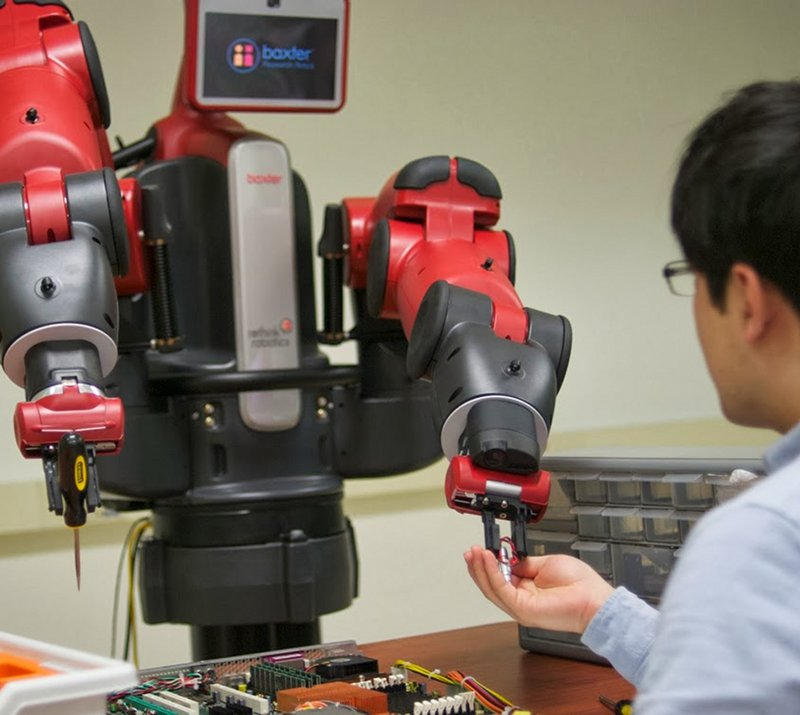
\includegraphics[width=0.3\linewidth]{images/baxter_scene_cropped.jpg}
\caption{Robots that collaborate with people need to understand their
  references to objects in the environment.  For example, if a person
  asks for a tool using language and gesture, the robot needs to
  interpret the person's reference in order to pick up the correct
  tool.\label{fig:example}}
\end{figure}

Despite the importance of a system capable of real-time response to multimodal input, existing models approaches fail to meet this high bar. Several systems focus on single modalities, which are insufficient to handle complicated interactions, such as ambigious phrases accompanied by gestures or vice versa~\citep{tellex11, kollar10}. Approaches that have incorporated multiple sources have failed to do so in an online manner, relying on batch interpretation, which is not fast enough for systems that need to respond immediately~\citep{matuszek14}. These approaches preclude rapid reaction, clarifying feedback, and the level of interpretation necessiated by human referring expressions.

To provide a foundation for these capabilities, we propose a Bayes' Filter to interpret information from language and gesture~\citep{thrun08}. Our framework relies on a factored observation probability that fuses information from language and gesture in real time to continuously estimate the object a human user is referencing. We initially demonstrate our model in simulation, and then perform user studies with our system running on a RGB-D corpus of untrained users referencing objects on a table. The results show that our model quickly and effectively fuses multimodal information in real time to continuously estimate the object being referenced. Additionally, we demonstrate a robot that uses our model to provide feedback in the form of facial expressions, pointing, and handing the user the object referenced in real time by interepreting gesture and language.

\begin{figure*}
\centering
\subfigure[Ambiguous gesture.\label{fig:confused}]{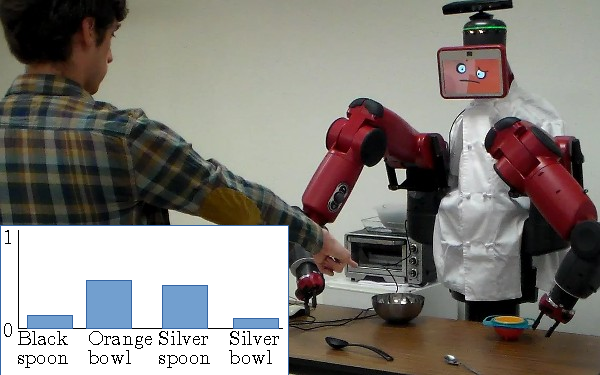
\includegraphics[width=0.49\linewidth]{images/cartoon1.pdf}}
\subfigure[Clarification with language.\label{fig:clarified}]{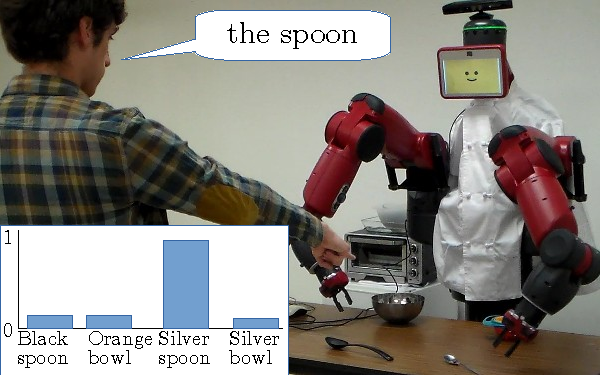
\includegraphics[width=0.49\linewidth]{images/cartoon2.pdf}}
\caption{After an ambiguous gesture, the model has a uniform
  distribution between two objects (a).  The robot responds by
  indicating confusion.  Clarification with language causes a
  probabilistic update leaving the model highly confident it has
  inferred the correct object (b).  The robot responds by smiling and
  pointing to the correct object. \label{fig:cartoon}}
\end{figure*}

\section{Related Work}
~\citep{clark96} proposed that conversation is a \textit{joint activity}, a coordinated, collaboraitve process in which the two participants establish \textit{common ground}. Common ground refers to the process by which each participant establishs an understanding about the beliefs of the other. In order to establish common ground, people use various forms of feedback, ranging from head nods to looks of confusion to explicit clarifying questions. These forms of feedback allows the participants to iteratively establish common ground through instruction and clarification as time progresses. Our Bayes' Filter approach provides a foundation for producing this feedback with a robot, which has the ability to increase robustness and reduce rate of error in human-robot communication through the establishment of common ground during interactions.

A large body of research focuses on language understanding for robots, ignoring information, but fails to account for the continuous nature of language, requiring full sentences or some other form of batching before interpretation can take place~\citep{macmahon06, dzifcak09, kollar10, matuszek12}. While this batching can help improve accuracy, the delays it imposes are unreasonable for a real time system. Our approach, in contrast, incorporates each word as it is processed during speech recognition, integrating it over time and fusing it with body language. In a similar vein as our research, \citet{guadarrama14} interprets open-domain references to objects, but still fails to include gesture, precluding natural non-verbal references. \citet{cantrell10} provides a framework for incrementally interpreting language, but neither includes language nor corpus based results. Our approach draws several ideas from each of these, but focuses on a more robust system of continuous understanding and interpretation.

Many other approaches for command interpretation depend on command words such as ``follow'' or ``stop''~\citep{waldherr00, marge11}. This type of system goes directly against what is desired, which is that an untrained user could interact with the system in whatever way felt most natural, rather than enforcing some small set of keywords that trigger specific behavior. This type of system removes the ability to make a robotic assistant to appear human in it's actions and reactions, and also ignores the importance of body language in interactions, as well as continuous interpretation of language.

\citet{matuszek14} presented work that falls closest to ours; a multimodal framework for interpreting unscripted references to tabletop objects using language and gesture, providing an accuracy rate comparable to the accuracy our system demonstrates in correctly indentifying the referenced object. However, this system relies on interpretation of batched data, failing to operate in real time, strictly limiting it in comparison to our continuous Bayes' Filter approach.

Partially Observable Markov Decision Process approaches to dialogue interpretation have been extended to incorporate gesture and noise models, similiar to our approach~\citep{young13, young10} . We have begun exploring similar methods of generating robot response, leading to informative feedback from a robotic assistant. \citet{dragan13} created a system to enable a robot to create gestures designed to strike a balance between legibility and predictibility. While we have explored the research in creating feedback, we have mostly focused on interpreting these gestures from humans, rather than generating them. Our long-term aim is to combine the understanding we have created with these systems to produce feedback, allowing for the rapid creation of common ground between a robotic assistant and a human user.
\section{Technical Approach}
Our aim is to estimate a distribution over which object a human user is referencing given language and body pose inputs. We frame this problem as a Bayes' Filter~\citep{thrun08}, where the \textit{hidden} state $x \in \mathcal{X}$ is the object in the scene the person is currently referencing. The robot observes the speech and gesture $z \in \mathcal{Z}$ at each timestep $t$ and continuously estimates a distribution over $x_t$, as shown in Figure~\ref{fig:model}. This model requires access to a transisition function specifying $p(x_t | x_{t-1})$ and an observation function specifying $p(z_t | x_t)$. Part of our model involves the development of these functions.

\begin{figure}[h]
\centering
\fbox{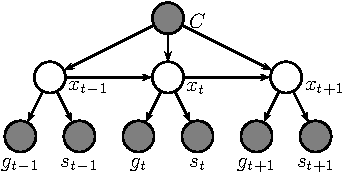
\includegraphics{images/bigram-crop.pdf}}
\caption{Graphical model for our approach with each observation factored into gesture ($g$) and speech ($s$). $C$ is the overall contextual information.\label{fig:model}}
\end{figure}

Formally, we wish to calculate:
\begin{align}
p(x_t | z_0, \dots, z_t)
\end{align}

To estimate this distribution, we perform alternating time and measurement updates. The time update incorporates the hidden state transitions using the previous state estimate and knowledge of the state transitions:
\begin{align}
p(x_t | z_{0:t-1}) = \int_{x_{t-1} \in \mathcal{X}} p(x_t|x_{t-1})\times p(x_{t-1} | z_{0:t-1}) \text{d}x_{t-1}
\end{align}

The measurement update combines the previous belief with the newest observation to update each belief state: 
\begin{align}
p(x_t |z_{0:t}) = \frac{p(z_t | x_t) \times p(x_t | z_{0:t-1})}{p(z_t | z_{0:t-1})} \\\propto p(z_t | x_t) \times p(x_t | z_{0:t-1})
\end{align}

Once normalized, this gives us an easily calculable, accurate estimation of the users state at each time step.
\subsection{Transition Model}
We assume that a person is likely to continue referring to the same
object, and so has a large probability $c$ of remaining in the state

\begin{align}
p(x_t | x_{t-1}) = \left\{  \begin{array}{ll}
c&\mbox{if } x_t = x_{t-1}\\
1-\frac{c}{|X|-1}&\mbox{otherwise}
\end{array}\right.
\end{align}

This assumption means that the robot's certainty slowly decays in the absence of meaningful observations, convergine to a uniform distribution. This enables our framework to find a balance between integrating past information and incorporating new, contrary information to switch the most likely estimated state.
\subsection{Observation Model}
We assume access to an observation model of the form:
\begin{align}
p(z_t | x_t)
\end{align}

Observations consist of a tuple consisting of a person's actions,
$\langle l, r, h, s\rangle $ (shown in Figure~\ref{fig:labeled_obs}) where:
\begin{itemize}
    \item $l$ represents a vector from the observed origin ($l_o$) to the point ($l_v$) of the left arm.
    \item $r$ represents a vector from the observed origin ($r_o$) to the point ($r_v$) of the right arm.
    \item $h$ represents a vector from the observed origin ($h_o$) to the point ($h_v$) of the head. This is the angle of the head transformed into a unit length vector.
    \item $s$ represents the observed speech from the user,
          consisting of a list of words.
    \end{itemize}

\begin{figure}[h]
\centering
\fbox{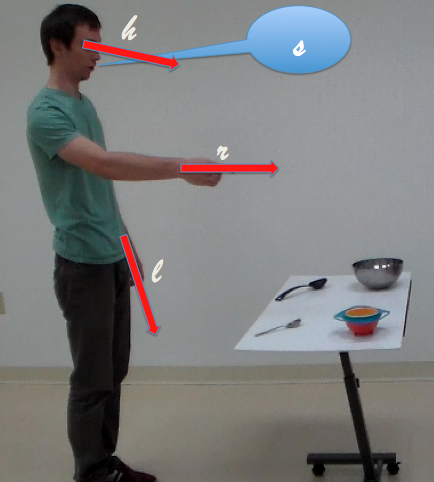
\includegraphics[scale=0.5]{images/labeled_obs.png}}
\caption{An image from our corpus with the components of observation labeled.\label{fig:labeled_obs}}
\end{figure}
Formally, we have:
\begin{align}
p(z_t | x_t) &= p(l, r, h, s | x_t)\\
\intertext{We factor assuming that each modality is conditionally independent of the others given the state (the true object that the person is referencing):}
p(z_t | x_t) &= p(l | x_t) \times p(r | x_t) \times p(h | x_t) \times p(s | x_t)
\end{align}
\subsubsection{Modeling Gesture}
We track body pose using the NITE skeleton tracker~\citep{openni}. We use this skeletal pose information to extract the 3D vector representing each forearm and the angle of the head (a unit length vector computed based on the observed rotation of the head). We then project the forearm gestures such that each arm vector actually originates in the wrist, as shown in Figure~\ref{fig:labeled_obs}. These three vectors comprise our deictic gestures.

To convert each vector observation $v$ into a probability for each object we need to compute $p(v | x_t)$. Since $v$ is composed of an origin $o$ and a point $p_1$, we simply take the center of mass of the object $x_t$, which we will call $p_2$. Next, we define a function $\mbox{A}(o, p_1, p_2)$ to calculate the angle between $p_1$ and $p_2$ using origin $o$. With this angle, we then calculate the density of a Gaussian  distribution $\mathcal{N}$ with zero mean and standard deviation $\sigma$ to convert the angle into a probability. Formally, this gives us:
\begin{align}
p(l | x_t) \propto \mathcal{N}(\mu_l=0, \sigma_l)[A(l_o, l_v, x_t)]\\
p(r | x_t) \propto \mathcal{N}(\mu_r=0, \sigma_r)[A(r_o, r_v, x_t)]\\
p(h | x_t) \propto \mathcal{N}(\mu_h=0, \sigma_h)[A(h_o, h_v, x_t)]
\end{align}
\subsubsection{Modeling Speech}
We model speech with a unigram model, namely we take each word in a given transcribed speech input and calculate the probability that, given the state, that word would have been spoken. Although a unigram model will often miss out on important combinations of words, such as ``blue bowl'' versus ``red bowl'', the continuous nature of the Bayes' Filter actually incorporates the combination of words in a meaningful way despite only using a unigram model, even if the color and the word ``bowl'' occur at different timesteps. Formally:
\begin{align}
p(s |x_t) = \displaystyle \prod_{w \in s} p(w | x_t)
\end{align}

To train these individual probabilities, we use a corpus of object-word associations. If word $w$ appeared in the corpus associated with object $x_t$ $k$ times out of $n$ total (not necessarily unique) words associated with $x_t$, then:
\begin{align}
p(w | x_t) = \frac{k}{n}
\end{align}
\subsubsection{Null Words and Gestures}
While the models for interpreting referring expressions discussed so far are accurate when interpreting meaningful gestures and speech, they encounter problems when there is meaningless speech or gestures, such as someone just repeating ``cake'' when there is no cake\footnote{The cake is a lie} or simply holding their arms by their sides. Expressions like this have the ability to zero all probabilities (in speech) or skew probabilities randomly even if one arm is pointing and the other is by a user's side. Throughout our user studies, we found that, especially with gesture, these types of meaningless expressions were common. To solve this problem for speech, we simply incorporated some basic epsilon smoothing, so that for object $x_t$ with an associated corpus of size $n$ in which word $w$ did not occur, rather than caculating:
\begin{align}
p(w | x_t) = \frac{0}{n} = 0
\end{align}

We calculate:
\begin{align}
p(w | x_t) = \epsilon = \frac{1}{n}
\end{align}

The meaningless gestures posed a more difficult problem. Initially we tried to solve this by calculating the angle between a gesture vector and the users feet. If that angle was smaller than the angle between the gesture and any object, then we simply applied equal weight to all objects, essentially treating it as a non-existent gesture. However, this caused problems with users crossing their arms, scratching an itch, and other innocuous movements. This is the method we used user studies, however, in later iterations we tried two different methods. The first involved simply treating a gesture as non-existent if it was greater than some angle $\theta$ away from all objects. This was easy to tune and performed fairly well, but in hope of greater robustness, we also implemented a third method of smoothing. This method involved replacing:
\begin{align}
p(v | x_t) \propto \mathcal{N}(\mu_l=0, \sigma_l)[A(v_o, v_v, x_t)]
\end{align}
With:
\begin{align}
p(v | x_t) \propto max(min\_prob, \mathcal{N}(\mu_v=0, \sigma_v)[A(v_o, v_v, x_t)])
\end{align}

This method of smoothing flattens the ends of the Gaussian distribution into constants, rather than continuing to decay regardless of the magnitude of the angle, as show in Figure~\ref{fig:gauss}\footnote{Image generated by wolframalpha.com}, avoiding the strange skewing that occured without the smoothing. This has proved more diffcult to tune appropriately, but avoids completely ignoring any gesture, and therefore seems to be more robust in the long term.
\begin{figure}[h]
\centering
\fbox{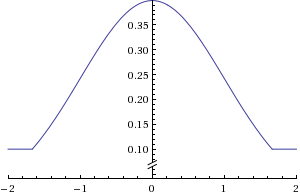
\includegraphics[scale=0.5]{images/gauss.png}}
\caption{A Gaussian distribution with uniform smoothing.\label{fig:gauss}}
\end{figure}
\subsection{Model Parameters}
We tuned model parameters by hand. We considered collecting and annotating a data set to train the model parameters, but we found that our initial process was quite accurate during real world trials. We generated the language model by hand, adding to it based on results of our pilot studies. After our initial tuning, we fixed model parameters for the duration of the user studies. 

In our experiments we had the following parameters:\begin{itemize}
\item The transition probability $c$, which was set to 0.985. We set this paramater to give an object that has near 100\% confidence an approximately 10\% drop in confidence per second with all null observations.
\item The standard deviations $sigma_l$, $sigma_r$, and $sigma_h$, used in the Gaussian distribution to convert gestures into probabilities. We found that $sigma_l = sigma_r = sigma_h = 1.0$ allowed for accurate pointing, without rapidly skewing the confidence distribution during an arm swing or slight meaningless motion.
\item The language model, which consisted of sixteen unique words, containing the most common decriptors for each of the objects such as ``bowl,'' ``spoon,'' ``metal,'' and ``plastic''. It also included words that were commonly misinterpreted by the speech recognition system, such as ``bull'' in place of ``bowl.'' For our user studies, this small, hand trained set was sufficient, but for larger trials with more object we intend to train language models on Amazon Mechanical Turk.
\item $\epsilon$, the smoothing factor for the unigram language model. Since our word corpus was so small, we decided to simply set $\epsilon$ to 0.0001 rather than the expected $\frac{1}{n}$ where $n$ is the size of the corpus. This was to simulate the effects of a larger corpus despite the size of our corpus. This is identical to simply duplicating the hand crafted data until the corpus contained 10,000 words.
\end{itemize}
\begin{algorithm}
    \DontPrintSemicolon
    \KwIn{$bel(x_{t-1}), z_t$}
    \BlankLine
    \KwOut{$bel(x_t)$}
    \BlankLine
    \For{ $x_t$} {
      $\bar{bel}(x_t) = \displaystyle\sum_{x_{t-1} \in \mathcal{X}} p(x_t|x_{t-1})*bel(x_{t-1})$
      \BlankLine
      \textbf{if not} is\_null\_gesture(l)
      \BlankLine
      \Indp$\bar{bel}(x_t) = p(l | x_t) *  \bar{bel}(x_t)$
      \BlankLine
      \Indm\textbf{if not} is\_null\_gesture(r)
      \BlankLine
      \Indp$\bar{bel}(x_t) = p(r | x_t) *  \bar{bel}(x_t)$
      \BlankLine
      \Indm\textbf{if not} is\_null\_gesture(h)
      \BlankLine
      \Indp$\bar{bel}(x_t) = p(h | x_t) *  \bar{bel}(x_t)$
      \BlankLine
      \Indm\For{$w \in s$}{
        $\bar{bel}(x_t) = p(w | x_t) *  \bar{bel}(x_t)$
      }
      $bel(x_t) = \bar{bel}(x_t)$
    }
    \BlankLine
\caption{Interactive Bayes Filtering Algorithm} 
\label{alg:algorithm}
\end{algorithm}

Algorithm~\ref{alg:algorithm} shows pseudocode for our approach, run once per timestep. 
By using this algorithm, our system is able to fuse speech and body lanaguage to continuously estimate the object being referenced by a human user, reacting quickly to new verbal and non-verbal information. This system runs at a rate of 14Hz, including a 30Hz sleep cycle, on an Asus machine with 8 2.4 GHz Intel Cores, while all perceptual and network processing inherenet in the Robot Operating System (ROS) are also being run on the same machine. This software is used in conjuction with the Baxter Robot, interfaced through ROS, and a Kinect V1.
\subsection{Assumptions}
Our Bayes Filter approach makes several simplifying assumptions. For clarity, we examine those assumptions here.

First, our algorithm assumes that referring expressions from humans are Markovian, namely that each observation depends only on the current state and that each state depends only on the previous state. This is not necessarily true, especially with long tasks with several sub-components that are linked. Despite this limitation, our real world results show that this is a reasonable simplifying assumption.

We assume that the system knows all objects in our environment. This includes not only location, but also models to enable picking and placing, as well as a corpus of words associated with each object. This is so that the focus of the success and error of this algorithm is restricted to the algorithm. There are ways to facilitate generation of these models `on the fly' \menote{cite ein?}, but doing so is out of the scope of this research.

We also assume that the forearm, as opposed to the fingers, are what generates a pointing gesture. Ideally, we would be able to use hand orientation to gain a better idea of the direction of a pointing gesture, as well as classify whether the hand was in a `pointing' pose. Unfortunately, we did not have access to hand tracking software that was sufficiently accurate at the distance we needed. If this software became available, it would be simple to incorporate it in place of the arms, but as of now, it is not.

Finally, we assume that all components of an observation are conditionally independent given the state. Namely, if it is known that a person wants a specific object, the probability that they point with their left hand and that they speak to indicate the object are independent. This is a simplyfing assumption intended to make the computation of $p(x_t | z_t)$ tractable. While it is not necessarily true, since a person is probably more likely to point and say ``hand me that'' than not point and say the same phrase, our user studies show that this is not a detrimental assumption to make.
\section{Evaluation}
We evaluated our model, comparing the full model to versions without multimodal information. We also assesed the algorithm's performance on an unscripted corpus of real-world audio and video data of human users referring to objects on a table. We used the results to compare the usefullness of various sources of referring expressions, as well as the efficacy of our system.
\subsection{Simulation Results}
We evaluated our approach in simulation by generating data from the model and accessing it's accuracy at estimating the object being referenced. We generated simulation data for spoken words, as well vectors for both arms and the head at each time step according to the model parameters by sampling from the distributions for each paramter. It is important to note that this means that no null gesture or speech was every generated. Five `objects' were randomly placed in a 10 by 10 by 10 cube. The word corpus for each object was randomly generated out of a small set of words. We then ran 100 simulated trials for 1000 time steps each, with the referenced object switching every 10 timesteps. To assess the robustness of the system to signal noise, we ran the same simulation with two different values as the gesture variance, $\sigma^2$, demonstrating that even with high levels of noise, the system can fuse multimodal information to improve accuracy. Table~\ref{table:sim_results} shows the accuracy of the system during these trials. Accuracy is measured as the percentage of time the algorithm's most likely object matched the true object being referenced.
\begin{table}[h]
\centering
\caption{Simulation Results\label{table:sim_results}}
\begin{tabular}{lcr}
\toprule
& $\sigma^2 = 0.5$ & $\sigma^2 = 1.0$\\
Language only &  36.5\% & 37\%\\
Head only & 50.9\% & 35.8\%\\
Arms only & 62.4\% & 42.1\%\\
Multimodal (all)&  65.7\% & 54.1\%\\
\bottomrule
\end{tabular}
\end{table}
\subsection{Real-World Corpus-Based Results}
\begin{figure}
\centering
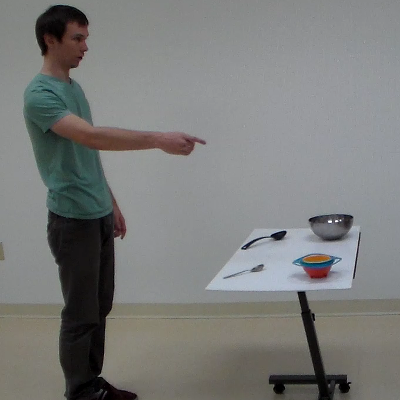
\includegraphics[width=0.5\linewidth]{images/dataset.png}
\caption{Scene from our data collection environment.\label{fig:corpus_scene}}
\end{figure}

We ran 65 user trials, consisting of 13 participants runnning 5 trials each to measure the algorithm's accuracy at estimating a human's referenced object when given real world RBG-D data and audio. Each subject stood in front of a table with four objects arranged to form a square, as appears in Figure~\ref{fig:corpus_scene}. The four objects used in these trials were a metal spoon, a plastic spoon, a metal bowl, and a plasic bowl. This was designed so that few single word descriptions would uniquely differentiate all the objects. We instructed each participant to ask for the object indicated with a laser pointer in whatever way felt most natural, using any combination of language or gesture. The participants wore a microphone to pick up quality audio for transcription. We used the HTML5 Webkit Audio API in conjuction with Google Chrome for speech transcription. This package supports incremental output as recognition proceeds, allowing us to update the model each time a new word is received, fitting in well with our continuous model.

Results showing the percent of the time the estimated most likely
object was the true object appear in Table~\ref{table:real_results}
with 95\% confidence intervals.  During a typical trial, the model
starts out approximately uniform or unimodal on the previous object
(we did not reset the model between trials for the same user) As the subject points and
talks, the model quickly converges to the correct object.  Our first
set of results give a sense of how quickly the model converges by measuring total time correct.

To assess overall accuracy, we report the system's accuracy at the end
of a trial in \ref{table:end_real}.  Multimodal accuracy with language
and gesture is more than 90\%, demonstrating that our approach is able
to quickly and accurately interpret unscripted language and gesture
produced by a user.  We found that our head pose estimator was quite
inaccurate, performing slightly below random.  Thus overall
results that include head pose perform worse than language and
gesture.  We believe this effect has several sources, including marginal head movement when objects are relatively close together, as well as general inaccuracy in head rotation tracking. 

The difference in accuracy between gesture alone and the multimodal output is not as large as one might expect. This is in part caused by the small delay in speech recognition software as opposed to the instantaneous gesture input. Additionally, many subjects, when told they could use gestures, leaned towards relying almost entirely on gesticulation. There were some users, however, who relied on an equal mix of both, and showed large leaps in accuracy between arms and multimodal. The most extreme example is of a user who, over their five trials, achieved only 45.5\% accuracy with arms alone and 42.2\% with speech alone, yet managed to achieve 85.7\% multimodal accuracy, only 2 percentage points away from the sum of the two probabilities, showing the ease at which alternating speech and gesture can give incredibly accurate results overall. While a combination of ambiguous speech and gesture such as "that spoon" followed by a gesture would be more accurate than just a gesture, we found that most test subjects either spoke with complete ambiguity or none, using phrases either of the form "hand me that thing" or "hand me the silver spoon". Therefore we were unable to fully test this hypothesis.
\begin{table}
\caption{Real-world Results\label{table:real_results}}
\centering
\begin{tabular}{lr}
\toprule
Random & 25\%\\
Language only &  32.4\% +/- 10\%\\
Gesture only  &  73.12\% +/- 9\%\\
Head only     &  21.67\% +/- 10\%\\
Multimodal (Language and Gesture) & {\bf 81.99\% +/- 5.5\%}\\
Multimodal (All) &  64.84\% +/- 8\%\\
\bottomrule
\end{tabular}
\end{table}
\begin{table}
\caption{Real-world Results (End of Interaction)\label{table:end_real}}
\centering
\begin{tabular}{lr}
\toprule
Random & 25\%\\
Language only &  46.15\%\\
Gesture only  &  80.0\%\\
Head only     & 18.46\%\\
Multimodal (Language and Gesture) & {\bf 90.77\%}\\
Multimodal (All) &  61.54\%\\
\bottomrule
\end{tabular}
\end{table}
\subsection{Sources of Error}
These trials have several sources of error, some caused by software, and some caused by the introduction of subjects to these trials.

The first, and most prominent, source of error is most likely the preconditioning felt by the test subjects. Test subjects were told what this system was intended to due, and upon hearing that the kinect tracked their gesture, many tended to use predominatly gestures. This could help explain why speech accuracy was so low compared to gesture accuracy. While this is a source of error, in the end, it simply demonstrates the versatility of this algorithm, regardless of what form of referring expression the human user is most comfortable with.

Another source of error is the accuracy of the skeleton tracker and it's calibration relative to the positioning of the objects. During our trials, we found that the skeleton tracker had a tendency to overlay a skeleton, as opposed to inserting it. Namely, the skeleton appeared to be projected on top of the skin rather than where one would expect the skeleton to be. This is the source of some inaccuracy, but from the user studies appears not to have had a detrimental effect. In addition to this, the positioning of objects and the Kinect needed to be calibrated to be in the same reference frame. Errors in this could have compounded this overlay problem.

Erroneous transcription of speech was a large source of error for the unigram model. We tried to mitigate this by including words that were commonly transcribed incorrectly, such as ``bull'' instead of ``bowl,'' however varying accents and speech paterns impacted the transcription process. This could be solved in the future by using large sets of spoken descriptions to train the unigram models, collected through Amazon Mechanical Turk or similar services.

The final major source of error was the lack of a hand tracker. Were we forced to rely on the forearm position for deictic gestures, which was reasonable enough given the software we had access to. This caused problems however, when people curved their wrists slightly during a pointing motion, as it often caused the system to interpret their gesture as pointing slightly behind the object the human user was intending to point at. This especially caused problems because our user study setup had objects behind each other, making the system interpret gestures to the closer objects as more ambigiuous than they were.

\section{Future Work}
There is much room to expand the capabilities of the system we have created, both improving its accuracy and its ability to perform more complex reasoning than simply determining the object currently being referenced.

To improve accuracy, we have several goals for future work. We currently make use of existing speech transcription software, relying on it to provide quick and reasonably accurate continuous transcription. To improve both the speed and reliability, we hope to be able to design an interface with more access to the interim results, so that instead of only incorporating the most likely transcription, we could incorporate the top 90\% of transcriptions, weighting each word according to its probability. This would increase accuracy and robustness of our speech transcription and incorporation. In addition, we could add a parsing chart to the state, which has the potential to allow the system to understand nested referring expressions such as ``the pen in the cup.''

The addition of hand tracking software would greatly improve accuracy. First, accuracy could be impoved with more fine-grained tracking, but we could also add a gesture classifier on top of the tracking, which would provide a confidence level that a given hand pose was a pointing gesture, allowing us to incorporate more accurate and weighted results into the Bayes' Filter.

While we found that head tracking was equivalent to noise during our trials, we believe that eye tracking software could be incorporated as a new modality to replace what we had hoped the head tracking would be. By following the eye movement, we gain a new source of information that could assist in more accurate determination of the referenced object.

These three components would greatly improve the accuracy of our system, while leaving the basic functionality untouched. To improve overall functionality and reasoning, we would need a more robust model built on top of the Bayes' Filter to perform higher reasoning about the world and what actions are appropriate.

To tackle this challenge, we have begun exploring the efficacy of a POMDP framework~\citep{kaelbling99}. This expands upon the Bayes' Filter approach by adding responsive actions the robotic agent can take to affect the world and user's state. In our original model, when interacting with the robot, we simply hard coded thresholds at which to perform certain actions, such as pointing, picking, smiling, etc. Once this POMDP system is in place, we imagine using a framework similar to that created by \citet{dragan13} for generating legible gestures. This would enable a robot to respond by pointing as in \citet{holladay14} when it is confident and reflect it's confusion through facial expressions or a variety of gestures when it is not. This would increase the efficiency of the establishment of common ground by naturally eliciting more information from both parties.

To make the system as a whole more robust, we hope to be able to incorporate object training and feature identification into the base functionality. Allowing the robot to learn features of objects and train objects `on the fly' would remove the current limitations that all object and object models must be known. This would a robotic assistant to move smoothly between a variety of tasks with similar, but not identical objects, which is necessary for a robotic assistant to be capable in a variety of real world situations.

Finally, we hope to expand the system beyond simple object references, allowing a wider variety of requests to be processed in a similar continuous fashion. While understanding object references is an important step, a wide variety of commands can be understood with some modifications to this framework, which would greatly increase its usability.
\section{Conclusion}
We have demonstrated a Bayes' Filtering approach to interpreting a person's natural language and gesture references to objects in the real world continuously in real time. Our approach not only allows for rapid understanding, but also for the easy simultaneous incorporation of various sources of input. This system provides a novel and extensible method of continuous interpretation and understanding of human referring expressions. This work represents a step towards real world human-robot interaction and the vision presented by \citet{clark96} of communication as joint activity. While there is still much work that can be done to improve this system, we have demonstrated it's effectiveness in real world situations with untrained users. By using this system, a robotic assistant can accurately interpret a human user's object references in real time.


\end{document}